% Lecture Template for ME3050 - Dynamic Modeling and Controls - Tennessee Technological University
% Spring 2024 - condensing and streamlining lectures by combining topics into a single PDF under the module name
% this will simplify file and link management as well as make lectures easier to use in class
% - added image/ to clean directory and reduce redundancy, specific to module for now  

% Module Name: - ODE Review
% Topic 1 - Definitions and Classification
% Topic 2 - Engineering Applications
% Topic 3 - Example

\documentclass[fleqn]{beamer} % for presentation (has nav buttons at bottom)

\usepackage{../dmc_lectures} % .sty in parent folder

\author{ME3050 - Dynamics Modeling and Controls}

\newcommand{\MNUM}{2\hspace{2mm}} % module number 
\newcommand{\moduletitle}{ODE Review}

\newcommand{\sectionItitle}{ODE Review}
\newcommand{\sectionIItitle}{Separation of Variables}
\newcommand{\sectionIIItitle}{The Trial Solution Method}

\newcommand{\sectionIsubsectionItitle}{Definitions and Classification}
\newcommand{\sectionIsubsectionIItitle}{Engineering Applications}
\newcommand{\sectionIsubsectionIIItitle}{Example}
%\newcommand{\sectionIsubsectionIVtitle}{Course Topics}

\newcommand{\sectionIIsubsectionItitle}{Review}
\newcommand{\sectionIIsubsectionIItitle}{Separation of Variables}
\newcommand{\sectionIIsubsectionIIItitle}{Example}
%\newcommand{\sectionIIsubsectionIVtitle}{-}

\newcommand{\sectionIIIsubsectionItitle}{Exponential Assumption}
\newcommand{\sectionIIIsubsectionIItitle}{Complementary Solution}
\newcommand{\sectionIIIsubsectionIIItitle}{Particular Solution}
\newcommand{\sectionIIIsubsectionIVtitle}{Apply Initial Conditions}
\newcommand{\sectionIIIsubsectionVtitle}{Summary - 3 Cases}

% custom box
\newsavebox{\mybox}

\title{Lecture Module - \moduletitle}

\date{Mechanical Engineering\vspc Tennessee Technological University}

\begin{document}

	\lstset{language=MATLAB,basicstyle=\ttfamily\small,showstringspaces=false}

	\frame{\titlepage \center\begin{framed}\Large \textbf{Module \MNUM - \moduletitle}\end{framed} \vspace{5mm}}

	% Module Outline
	\begin{frame} 
		\large \textbf{Module \MNUM - \moduletitle} \vspace{3mm}\\

		\begin{itemize}
			\item Topic 1 - \hyperlink{sectionI}{\sectionItitle} \vspc % section I
			\item Topic 2 - \hyperlink{sectionII}{\sectionIItitle} \vspc % section II
			\item Topic 3 - \hyperlink{sectionIII}{\sectionIIItitle} \vspc % section III
		\end{itemize}

	\end{frame}

	% section I
	\section{\sectionItitle}\label{sectionI}

		% section I Outline
		\begin{frame} 
			\large \textbf{Topic 1 - \sectionItitle} \vspace{3mm}\\

			\begin{itemize}
				\item \hyperlink{sectionIsubsectionI}{\sectionIsubsectionItitle} \vspc %  section I subsection I
				\item \hyperlink{sectionIsubsectionII}{\sectionIsubsectionIItitle} \vspc % section I subsection II
				\item \hyperlink{sectionIsubsectionIII}{\sectionIsubsectionIIItitle} \vspc % section I subsection III
				%\item \hyperlink{sectionIsubsectionIV}{\sectionIsubsectionIVtitle} \vspc % section I subsection IV
			\end{itemize}
		\end{frame}
		
		% section I subsection I 
		\subsection{\sectionIsubsectionItitle}\label{sectionIsubsectionI}

			\begin{frame}
				\frametitle{\sectionIsubsectionItitle}
				\bigskip

 				\frametitle{What is a Differential Equation?}
  				{\it Definition:\vspace{3mm}\\}
  				A {\bf differential equation} is an equation which describes a function \vspace{3mm}\\and one or more of its \underline{\hspace{50mm}} of the \vspace{3mm}\\ \underline{\hspace{50mm}}\hspace{3mm}\underline{\hspace{50mm}}\vspace{5mm} \\ with respect to the \underline{\hspace{60mm}}.
	
				\btVFill
			\end{frame}

			\begin{frame}
				\frametitle{\sectionIsubsectionItitle}
				\bigskip

				  \frametitle{Standard Form of an ODE}

				  Ordinary Differential Equations are written in the following form.\vspace{3mm}\\

				\scalebox{1.2}{$a_n\frac{dy^{(n)}}{d^{(n)}x}+a_{n-1}\frac{dy^{(n-1)}}{d^{(n-1)}x}+...+a_{2}\frac{dy^{2}}{d^{2}x}+a_{1}\frac{dy}{dx}+a_0y=f(x)$}	\vspace{0mm}\\		

				The apostrophe is commonly used for the derivative. \vspace{2mm}\\

				\scalebox{1.2}{$a_ny^{(n)}+a_{n-1}y^{(n-1)}+...+a_2y'' +a_1y'+a_0y=f(x)$} \vspace{3mm}\\

				If time is the independent variable the equation changes slightly. \vspace{2mm}\\
 
  
				\btVFill
			\end{frame}

			\begin{frame}
				\frametitle{\sectionIsubsectionItitle}
				\bigskip

				\frametitle{Is the differential equation ordinary or partial?}

				An {\bf ordinary} differential equation has \underline{\hspace{20mm}} independent \vspc variable and \underline{\hspace{20mm}} dependent variable. \vspace{10mm}\\

				A {\bf partial} differential equation has \underline{\hspace{50mm}} \vspc independent variable  \underline{\hspace{20mm}}  dependent variable. \vspace{10mm}\\

				\btVFill
			\end{frame}

			\begin{frame}
				\frametitle{\sectionIsubsectionItitle}
				\bigskip

  				\frametitle{What is the order of the equation?}
  
				The {\bf order} of a differential equation is the \vspace{3mm}\\ \underline{\hspace{50mm}}\hspace{3mm}\underline{\hspace{50mm}} \vspace{5mm}\\ present in the equation. \vspace{3mm}\\
	  
				\btVFill
			\end{frame}

							\begin{frame}
				\frametitle{\sectionIsubsectionItitle}
				\bigskip

  				\frametitle{What is the degree of the equation?}

				The {\bf degree} of a differential equation is the \underline{\hspace{30mm}}\hspace{3mm} \vspace{5mm}\\ of its highest derivative, after the equation has been made rational \vspace{5mm}\\ and integral in all of its derivatives. \vspace{3mm}\\

				\btVFill
			\end{frame}

			\begin{frame}
				\frametitle{\sectionIsubsectionItitle}
				\bigskip

				\frametitle{Is the differential equation linear or non-linear?}

				An ordinary differential equation is \underline{\hspace{30mm}} if the following statements are true. \vspace{5mm}\\

				\begin{enumerate}
				\item {\it The dependent variable and its derivatives are of the first degree.} \vspace{3mm}\\

				\item {\it The coefficients are constants or dependent on the independent variable.}\vspace{3mm}\\
				\end{enumerate}

				If either rule is broken, the equation is \underline{\hspace{10mm}}-\underline{\hspace{30mm}}.
				  
				\btVFill
			\end{frame}



		% section I subsection II
		\subsection{\sectionIsubsectionIItitle}\label{sectionIsubsectionII}

			\begin{frame}
				\frametitle{\sectionIsubsectionIItitle}
				\bigskip

					\frametitle{Engineering Applications}

					Differential equations are used to describe physical systems in many areas of engineering. An equation that represents a physical (or theoretical) system is known as a \underline{\hspace{50mm}}\hspace{3mm}\underline{\hspace{50mm}}.\vspace{3mm}\\
					\begin{itemize}

						\item Solid Mechanics \vspace{3mm}\\
						\item Kinematics and Dynamics \vspace{3mm}\\
						\item Heat Transfer and Thermodynamics \vspace{3mm}\\
						\item Fluid Mechanics
								
					\end{itemize}
			
				\btVFill
			\end{frame}

				%\btVFill
			\begin{frame}
				\frametitle{\sectionIsubsectionIItitle}
				\bigskip
				

				  
		
				\btVFill
			\end{frame}

		% section I subsection III
		\subsection{\sectionIsubsectionIIItitle}\label{sectionIsubsectionIII}
			\begin{frame} 
				\frametitle{\sectionIsubsectionIIItitle}
				\bigskip

				\begin{multicols}{2}

					Newton's Second Law \vspace{2mm}\\

					$\Sigma {\bf F}=m {\bf a}$ \vspace{2mm}\\

					leads  to an {\it equation of motion}.  \vspace{2mm}\\

					$\dot{y}+\frac{c}{m}y=f(t)$

					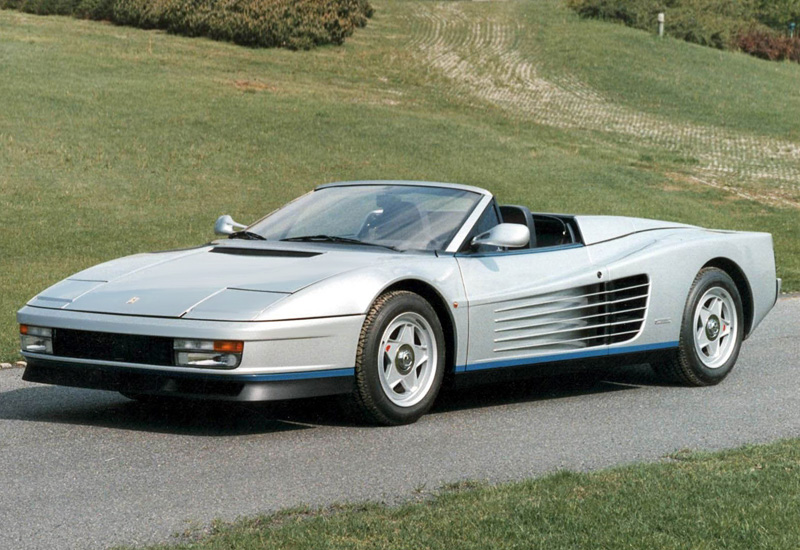
\includegraphics[scale=0.15]{images/ferrari.jpg}\\
				 
				\end{multicols} 	
				
				\btVFill
			\end{frame}	

	
	% Section II
	\section{\sectionIItitle}\label{sectionII}

		% section II Outline
		\begin{frame}
			\large \textbf{Topic 2 - \sectionIItitle} \vspace{3mm}\\

			\begin{itemize}
				\item \hyperlink{sectionIIsubsectionI}{\sectionIIsubsectionItitle} \vspc %  section II subsection I
				\item \hyperlink{sectionIIsubsectionII}{\sectionIIsubsectionIItitle} \vspc % section II subsection II
				\item \hyperlink{sectionIIsubsectionIII}{\sectionIIsubsectionIIItitle} \vspc % section II subsection III
				%\item \hyperlink{sectionIIsubsectionIV}{\sectionIIsubsectionIVtitle} \vspc % section II subsection IV
			\end{itemize}

		\end{frame}

		% section II subsection I
		\subsection{\sectionIIsubsectionItitle}\label{sectionIIsubsectionI}

			\begin{frame}[label=sectionIIsubsectionI]
				\frametitle{\sectionIIsubsectionItitle}
				\bigskip

				  \frametitle{What is a Differential Equation? Solution?}

A {\bf differential equation} is an equation which describes a function \vspace{3mm}\\and one or more of its \underline{\hspace{50mm}} of the \vspace{3mm}\\ \underline{\hspace{50mm}}\hspace{3mm}\underline{\hspace{50mm}}\vspace{2mm}\\ with respect to the \underline{\hspace{60mm}}. \vspace{8mm} \\
 
The {\bf solution} to a differential equation describes the \vspace{2mm}\\ \underline{\hspace{40mm}}\hspace{2mm}\underline{\hspace{40mm}} as a function \vspace{2mm}\\of the \underline{\hspace{40mm}}\hspace{2mm}\underline{\hspace{40mm}}.  \vspace{5mm}\\
				
				
				\btVFill
			\end{frame}


		% section II subsection II
		\subsection{\sectionIIsubsectionIItitle}\label{sectionIIsubsectionII}

		

	
			\begin{frame}

				\frametitle{\sectionIIsubsectionIItitle}
				\bigskip

				Separation of Variables: {\bf analytical} for solving differential equations \vspace{2mm}\\

				\begin{itemize}

					\item Step 1 - Separate\vspace{15mm}\\

					\item Step 2 - Integrate\vspace{15mm}\\
				
					\item Step 2 - Solve for Unknowns\vspace{15mm}\\
				
				\end{itemize}


				\btVFill 
			\end{frame}

			\begin{frame}

				\frametitle{\sectionIIsubsectionIItitle}
				\bigskip

				Alternative methods to find solution:

				\begin{itemize}

					\item - \vspace{10mm}\\

					\item - \vspace{10mm}\\
				
					\item - \vspace{10mm}\\
				
				\end{itemize}


				\btVFill 
			\end{frame}




		% section II subsection III
		\subsection{\sectionIIsubsectionIIItitle}\label{sectionIIsubsectionIII}

			\begin{frame}
				\frametitle{\sectionIIsubsectionIIItitle}
				\bigskip

				\frametitle{Problem Statement}

				Remember our example from the previous lecture?\vspace{5mm}\\

        		\scalebox{1.25}{$\dot{v}+\frac{c}{m}v=f(t)$} \vspace{2mm}\\
	
				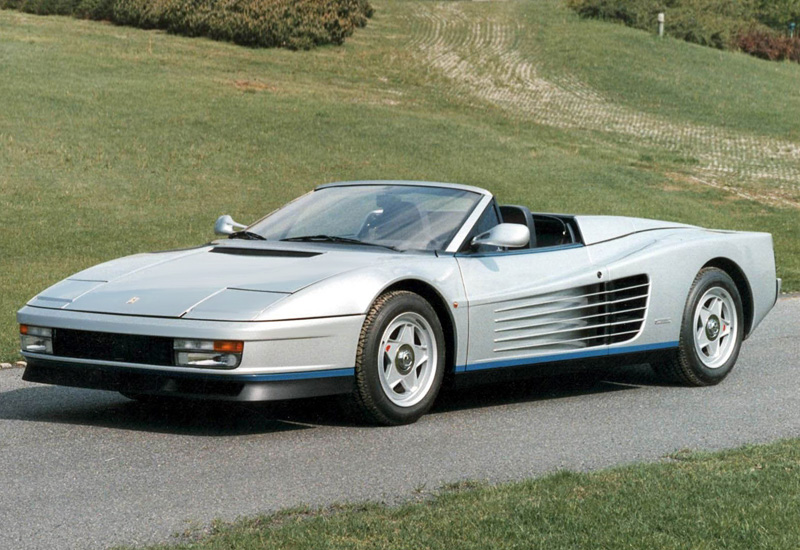
\includegraphics[scale=0.15]{images/ferrari.jpg} \hspace{10mm} \includegraphics[scale=0.10]{images/lecture1_fig2.png}\vspace{2mm}\\
	
				We are going to find an {\bf analytical solution} to this problem. 
  
				\btVFill 
			\end{frame}	


			\begin{frame}
				\frametitle{\sectionIIsubsectionIItitle}
				\bigskip

				\frametitle{Separation of Variables}

				Assume the external force $f(t)$ is zero. Use separation of variables to find the solution $v(t)$.  \vspace{5mm}\\

				\scalebox{1.25}{$\dot{v}+\frac{c}{m}v=0$} \vspace{50mm}\\
				
				\btVFill 
			\end{frame}	


			\begin{frame}
				\frametitle{\sectionIIsubsectionIIItitle}
				\bigskip

				\frametitle{Solution}

				The solution $v(t)$ has been found. What does it mean? What do we do next?\vspace{5mm}\\

				\scalebox{1.25}{$v(t)=$} \vspace{50mm}\\

				\btVFill 
			\end{frame}

			\begin{frame}
				\frametitle{\sectionIIsubsectionIIItitle}
				\bigskip

				\frametitle{Solution}

				The solution $v(t)$ has been found. What does it mean? What do we do next?\vspace{5mm}\\

				\scalebox{1.25}{$v(t)=$} \vspace{50mm}\\

				\btVFill 
			\end{frame}

			\begin{frame}
				\frametitle{\sectionIIsubsectionIIItitle}
				\bigskip

				\frametitle{Graph of Solution}

				What does the solution look like?\vspace{5mm}\\
				\scalebox{1.25}{$v(t)=v_0e^{-\frac{c}{m}t}$} \vspace{5mm}\\

				\includegraphics[scale=0.15]{images/lecture1_fig2.png}\hspace{5mm}%\includegraphics[scale=0.15]{lecture1_fig2.png}
				

				\btVFill 
			\end{frame}


		
	% Section III
	\section{\sectionIIItitle}\label{sectionIII}

		% section III Outline
		\begin{frame}
			\large \textbf{Topic 3 - \sectionIIItitle} \vspace{3mm}\\

			\begin{itemize}
				\item \hyperlink{sectionIIIsubsectionI}{\sectionIIIsubsectionItitle} \vspc %  section III subsection I
				\item \hyperlink{sectionIIIsubsectionII}{\sectionIIIsubsectionIItitle} \vspc % section III subsection II
				\item \hyperlink{sectionIIIsubsectionIII}{\sectionIIIsubsectionIIItitle} \vspc % section III subsection III
				\item \hyperlink{sectionIIIsubsectionIV}{\sectionIIIsubsectionIVtitle} \vspc % section III subsection IV
				\item \hyperlink{sectionIIIsubsectionV}{\sectionIIIsubsectionVtitle} \vspc % section III subsection V
			\end{itemize}

		\end{frame}

		% section III subsection I
		\subsection{\sectionIIIsubsectionItitle}\label{sectionIIIsubsectionI}

			\begin{frame}
				\frametitle{\sectionIIIsubsectionItitle}
				\bigskip


\frametitle{Trial Solution Method}
Use the {\bf trial solution method} to solve the ODE. \vspace{2mm}\\
This is an {\bf analytical} method that you learned in calculus but it may have been called something different. In the Zill book it is called {\it Homogenous Linear ... Constant Coefficients (4.3-4.4)}. \vspcc

\[a_2y''+a_1y'+a_0y=f(x)\] 
				

				\btVFill
			\end{frame}

			\begin{frame}
				\frametitle{\sectionIIIsubsectionItitle}
				\bigskip
				

				\btVFill
			\end{frame}

		% section III subsection II
		\subsection{\sectionIIIsubsectionIItitle}\label{sectionIIIsubsectionII}	

			\begin{frame}
				\frametitle{\sectionIIIsubsectionIItitle}
				\bigskip

				\underline{Step 1} - Find the {\bf complementary part} of the solution from the \vspace{1mm}\\ left hand side of the ODE alone (LHS=0). \\

				\[a_2y''+a_1y'+a_0y=f \hspace{5mm}\rightarrow\hspace{5mm} a_2y''+a_1y'+a_0y=0\] 

				Assume an exponential solution for the complementary part. \[y_{complementary}=y_c(x)=\] 

				Substitute this solution into the ODE (LHS=0).
				
				\btVFill
			\end{frame}

		% section III subsection III
		\subsection{\sectionIIIsubsectionIIItitle}\label{sectionIIIsubsectionIII}

			\begin{frame}
				\frametitle{\sectionIIIsubsectionIIItitle}
				\bigskip

				\underline{Step 2} - Find the {\bf particular part} of the solution from the entire equation (LHS=RHS). \vspcc  
				\[a_2y''+a_1y'+a_0y=f\] 

				The {\it form of the particular part} follows the RHS of  the ODE. \vspc

				\[y_{particular}=y_p(x)=\]  

				Substitute this solution into the ODE above and solve for any unknown constants in $ y_p(x) $. 
								
				\btVFill
			\end{frame}

		% section III subsection IV
		\subsection{\sectionIIIsubsectionIVtitle}\label{sectionIIIsubsectionIV}	

			\begin{frame}
				\frametitle{\sectionIIIsubsectionIVtitle}
				\bigskip

				\underline{Step 3} - Now combine the {\bf complementary} and {\bf particular} solutions through {\it superposition}. \\

				\[y(x)=y_c(x)+y_p(x)=\] 

				The ODE is first order and we have \underline{\hspace{10mm}} unknown. Coincidence?\vspcc

				\[y(x)=\]  

				This {\bf initial value problem} requires \underline{\hspace{10mm}} intial condition.\vspace{2mm}\\
				
				\btVFill 
			\end{frame}

			\begin{frame}
				\frametitle{\sectionIIIsubsectionIVtitle}
				\bigskip

				\[y(x=0)=\] 
				\[y'(x=0)=\] 

		 		\btVFill 
			\end{frame}
			
			\begin{frame}
				\frametitle{\sectionIIIsubsectionIVtitle}
				\bigskip
					What does the solution look like this time?\\

				\[y(x)=\] 

				\includegraphics[scale=0.15]{images/lecture1_fig2.png}\hspace{5mm} \includegraphics[scale=0.15]{images/lecture1_fig2.png}
				
				\btVFill 
			\end{frame}

			\begin{frame}
				\frametitle{\sectionIIIsubsectionIVtitle}
				\bigskip

				
				
				
				\btVFill 
			\end{frame}

		% section III subsection V
		\subsection{\sectionIIIsubsectionVtitle}\label{sectionIIIsubsectionV}	

			\begin{frame}
				\frametitle{\sectionIIIsubsectionVtitle}
				\bigskip

				If the differential equation is first and linear, the complementary solution takes the following form. \\

				\[y(x)=Ae^{sx}\] 

				\btVFill 
			\end{frame}

			\begin{frame}
				\frametitle{\sectionIIIsubsectionVtitle}
				\bigskip

				If the differential equation is second order and linear, the {\bf complementary solution } takes one of the following forms. \vspace{2mm}\\

				Case 1: $s_1,s_2\in\mathbb{R} \hspc,\hspc s_1\neq s_2$ 
				\[y(x)=c_1e^{s_1x}+c_2e^{s_2x}\] \vspace{2mm}
				Case 2: $s_1,s_2\in\mathbb{R} \hspc,\hspc s_1=s_2=s$
				\[y(x)=c_1e^{sx}+c_2xe^{sx}\] \vspace{2mm}
				Case 3: $s_1,s_2\notin\mathbb{R} \hspc,\hspc s_1,s_2 = \alpha\pm\beta$
				\[y(x)=e^{\alpha x}\left(c_1 cos\left(\beta x\right)+c_2 sin\left(\beta x\right) \right)\]
				
				\btVFill 
			\end{frame}

			\begin{frame}
				\frametitle{\sectionIIIsubsectionVtitle}
				\bigskip

				The {\bf particular solution} takes the form of the right hand side of the equation. \vspace{2mm}\\ 
				\renewcommand{\arraystretch}{1.5}
				\begin{tabular}{|c|c|c|}
					
					Example & Form & Particular Solution \\ \hline
					
					$... = 10$   & Constant & $y_p=B$ \\
					$... = 12x$  & Linear   & $y_p=Bx+C$\\
					$... = 20e^{2x} $ & Exponential & $y_p=Be^{2x}$ \\
					$... = a cos\left(\beta x\right)$& Sinusoidal &$ Bcos\left(\beta x\right)+Csin\left(\beta x\right)$ \\
					$... = a sin\left(\beta x\right)$& Sinusoidal &$ Bcos\left(\beta x\right)+Csin\left(\beta x\right)$ \\
					
				\end{tabular}

				
				\btVFill 
			\end{frame}

\end{document}





